%%%%%%%%%%%%%%%%%%%%%%%%%%%%%%%%%%%%%%%%%%%%%%%%%%%%%%%%%%%%%%%%
%%                                                            %%
%%   essentialsOfLatin, Italian translation 2017              %%
%%                                                            %%
%% From:  Henry C. Pearson, Essentials Of Latin For Beginners %%
%%        (1915, New York, American Book Company)             %%
%%                                                            %%
%%    https://archive.org/details/essentialslatin04peargoog   %%
%%                                                            %%
%% Translated by g.p.ciceri <gp.ciceri@gmail.com>             %%
%% ---------------------------------------------------------- %%
%% This translation is Licensed under                         %%
%% Creative Commons Attribution-ShareAlike 4.0 International  %%
%% https://creativecommons.org/licenses/by-sa/4.0/            %%
%%                                                            %%
%%%%%%%%%%%%%%%%%%%%%%%%%%%%%%%%%%%%%%%%%%%%%%%%%%%%%%%%%%%%%%%%

% āēīōū
% ăĕĭŏŭ




\documentclass[nols]{tufte-handout}

%\geometry{showframe} % display margins for debugging page layout

\usepackage{fontspec}
\usepackage{ifxetex}
\setmainfont[Path=./fonts/palatino-linotype/, ItalicFont=palai.ttf, BoldFont=palab.ttf]{pala.ttf}


% \defaultfontfeatures{Mapping=tex-text}
% \setromanfont[Path=./fonts/TeX-Gyre-Schola/,Mapping=tex-text]{TeX Gyre Schola}
% \setsansfont[Path=./fonts/TeX-Gyre-Heros/,Scale=MatchLowercase,Mapping=tex-text]{TeX Gyre Heros}
% \setmonofont[Path=./fonts/TeX-Gyre-Cursor/,Scale=MatchLowercase]{TeX Gyre Cursor}

\usepackage{lipsum}
\usepackage{url}
\usepackage{longtable}
\usepackage{stackengine}

\usepackage{graphicx} % allow embedded images
  \setkeys{Gin}{width=\linewidth,totalheight=\textheight,keepaspectratio}
  \graphicspath{{graphics/}} % set of paths to search for images
\usepackage{amsmath}  % extended mathematics
\usepackage{booktabs} % book-quality tables
\usepackage{units}    % non-stacked fractions and better unit spacing
\usepackage{multicol} % multiple column layout facilities
\usepackage{lipsum}   % filler text
\usepackage{fancyvrb} % extended verbatim environments
  \fvset{fontsize=\normalsize}% default font size for fancy-verbatim environments

% Standardize command font styles and environments
\newcommand{\doccmd}[1]{\texttt{\textbackslash#1}}% command name -- adds backslash automatically
\newcommand{\docopt}[1]{\ensuremath{\langle}\textrm{\textit{#1}}\ensuremath{\rangle}}% optional command argument
\newcommand{\docarg}[1]{\textrm{\textit{#1}}}% (required) command argument
\newcommand{\docenv}[1]{\textsf{#1}}% environment name
\newcommand{\docpkg}[1]{\texttt{#1}}% package name
\newcommand{\doccls}[1]{\texttt{#1}}% document class name
\newcommand{\docclsopt}[1]{\texttt{#1}}% document class option name
\newenvironment{docspec}{\begin{quote}\noindent}{\end{quote}}% command specification environment

% concetti morfosintattici
\usepackage{xspace} 
\newcommand{\noun}{\textsc{sostantivo}\xspace}
\newcommand{\nouns}{\textsc{sostantivi}\xspace}
\newcommand{\adject}{\textsc{aggettivo}\xspace}
\newcommand{\adjects}{\textsc{aggettivi}\xspace}
\newcommand{\gnumber}{\textsc{numero}\xspace}
\newcommand{\gnumbers}{\textsc{numeri}\xspace}
\newcommand{\gender}{\textsc{genere}\xspace}
\newcommand{\genders}{\textsc{generi}\xspace}
\newcommand{\gcase}{\textsc{caso}\xspace}
\newcommand{\gcases}{\textsc{casi}\xspace}
\newcommand{\tense}{\textsc{tempo}\xspace}
\newcommand{\mood}{\textsc{modo}\xspace}
\newcommand{\gverb}{\textsc{verbo}\xspace}
\newcommand{\gverbs}{\textsc{verbi}\xspace}
\newcommand{\adjective}{\textsc{aggettivo}\xspace}
\newcommand{\nom}{\textsc{nom}\xspace}
\newcommand{\gen}{\textsc{gen}\xspace}
\newcommand{\dat}{\textsc{dat}\xspace}
\newcommand{\acc}{\textsc{acc}\xspace}
\newcommand{\voc}{\textsc{voc}\xspace}
\newcommand{\abl}{\textsc{abl}\xspace}
\newcommand{\gexit}{\textsc{uscita}\xspace}
\newcommand{\gexits}{\textsc{uscite}\xspace}
\newcommand{\declinazione}{\textsc{declinazione}\xspace}
\newcommand{\masc}{\textsc{maschile}\xspace}
\newcommand{\femm}{\textsc{femminile}\xspace}
\newcommand{\neut}{\textsc{neutro}\xspace}

\newcommand{\indic}{\textsc{indicativo}\xspace}
\newcommand{\imper}{\textsc{imperativo}\xspace}
\newcommand{\gcong}{\textsc{congiuntivo}\xspace}
\newcommand{\ott}{\textsc{ottativo}\xspace}
\newcommand{\partic}{\textsc{participio}\xspace}
\newcommand{\infin}{\textsc{infinito}\xspace}

\newcommand{\pres}{\textsc{presente}\xspace}
\newcommand{\imperf}{\textsc{imperfetto}\xspace}
\newcommand{\aor}{\textsc{aoristo}\xspace}
\newcommand{\fut}{\textsc{futuro}\xspace}
\newcommand{\perf}{\textsc{perfetto}\xspace}
\newcommand{\pperf}{\textsc{piuccheperfetto}\xspace}

\newcommand{\sing}{\textsc{singolare}\xspace}
\newcommand{\plur}{\textsc{plurale}\xspace}
\newcommand{\dual}{\textsc{duale}\xspace}

\newcommand{\si}{\textsc{sing}\xspace}
\newcommand{\pl}{\textsc{plur}\xspace}
\newcommand{\du}{\textsc{dual}\xspace}

\newcommand{\att}{\textsc{attivo}\xspace}
\newcommand{\med}{\textsc{medio}\xspace}
\newcommand{\pass}{\textsc{passivo}\xspace}
\newcommand{\medpass}{\textsc{medio-passivo}\xspace}


% italianitudini
\renewcommand{\figurename}{Figura}
\renewcommand{\tablename}{Tabella}
\renewcommand{\contentsname}{Indice}

% fix per un qualche problema
\ifxetex
  \newcommand{\textls}[2][5]{%
    \begingroup\addfontfeatures{LetterSpace=#1}#2\endgroup
  }
  \renewcommand{\allcapsspacing}[1]{\textls[15]{#1}}
  \renewcommand{\smallcapsspacing}[1]{\textls[10]{#1}}
  \renewcommand{\allcaps}[1]{\textls[15]{\MakeTextUppercase{#1}}}
  \renewcommand{\smallcaps}[1]{\smallcapsspacing{\scshape\MakeTextLowercase{#1}}}
  \renewcommand{\textsc}[1]{\smallcapsspacing{\textsmallcaps{#1}}}
\fi

% too many float...
\extrafloats{100}
% āēīōū
% ăĕĭŏŭ

\title{Essentials Of Latin. Elementi di Latino. \newline Lezione IX - Seconda Declinazione (continua). nomi in -ius e -ium. Aggettivi in -er, (-e)ra, (-e)rum}

\author[gpciceri]{a cura di Milagathòs: Milo's help to enjoy humanities.}

\date{22 Febbrajo 2017} % without \date command, current date is supplied


\begin{document}

\hyphenation{co-niu-ga-zio-ne}

\maketitle% this prints the handout title, author, and date

\begin{marginfigure}[-2.5cm]
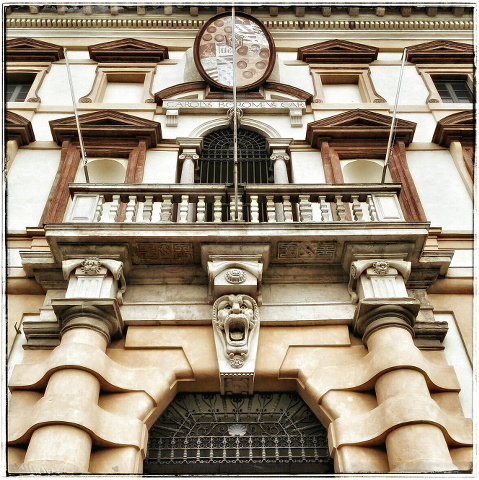
\includegraphics{smallthumb-lesson_I.jpeg}
\setfloatalignment{b}
\end{marginfigure}


\begin{abstract}
\noindent
Queste lezioni riprendono il testo introduttivo al Latino di Pearson\cite{pearson1915}, del quale seguono la numerazione; la struttura di ogni lezione è piuttosto regolare: inizia con \textsc{cenni di morfologia e di sintassi latina}, seguita da un \textsc{piccolo vocabolario} per il lessico; ci sono infine vari \textsc{esercizi} di traduzione e di composizione latina.

\bigskip
\noindent
Lezione IX - Seconda Declinazione (continua). nomi in -ius e -ium. Aggettivi in -er, (-e)ra, (-e)rum. Vocaboli, esercizi, lettura.
\end{abstract}

%\printclassoptions

% āēīōū
% ăĕĭŏŭ

\newthought{74. Seconda Declinazione, nomi in -ius e -ium.} \textbf{filius}, \textit{figlio}. Radice \textbf{fīlio-}, tema \textbf{fīli-}; 
\textbf{proelium}, \textit{battaglia}. Radice \textbf{proelio-}, tema \textbf{proeli-}.

\begin{fullwidth}
\begin{table}[!htbp]
  \centering
  \begin{tabular}{l l l }
    %\toprule
	& \multicolumn{2}{c}{\textsc{Singolare}} \\

    \nom & fīli\textbf{us} & proeli\textbf{um}  \\
    \gen & fīl\textbf{ī} (fīli\textbf{ī})  & proel\textbf{ī} (proeli\textbf{ī})  \\
    \dat & fīli\textbf{ō}  & proeli\textbf{ō}  \\
    \acc & fīli\textbf{um} & proeli\textbf{um} \\
    \voc & fīl\textbf{ī}   & proeli\textbf{um}              \\
    \abl & fīli\textbf{ō}  & proeli\textbf{ō}  \\
	
	\multicolumn{3}{c}{\textemdash} \\
	
	& \multicolumn{2}{c}{\textsc{Plurale}} \\
	
	\nom & fīli\textbf{ī} & proeli\textbf{a}  \\
    \gen & fīli\textbf{ōrum}  & proeli\textbf{ōrum}  \\
    \dat & fīli\textbf{īs}  & proeli\textbf{īs}  \\
    \acc & fīli\textbf{um} & proeli\textbf{a} \\
    \voc & fīli\textbf{ī}   & proeli\textbf{a}              \\
    \abl & fīli\textbf{īs}  & proeli\textbf{īs}  \\
	
    %\bottomrule
  \end{tabular}
  %\caption[bottom]{Prima Declinazione. \textbf{stella, -ae}, f.}
  \label{tab:normaltab}
  %\zsavepos{pos:normaltab}
\end{table}
\end{fullwidth}

\begin{itemize}
\item[\textsc{1.}] Il genitivo singolare dei nomi in \textbf{-ius} e \textbf{-ium} termina in genere in \textbf{-ī} (non in \textbf{-iī}). 
L'accento rimane sulla stessa sillaba del nominativo: \textbf{cōnsìlium}, \textit{piano}; \gen \textbf{cōnsìlī}.  
\item[\textsc{2.}] Nei nomi propri in \textbf{-ius} e in \textbf{filius}, il vocativo singolare esce in \textbf{-ī: fīlī}, \textit{o figlio}; 
\textbf{Mercurius}, \voc \textbf{Mercùrī}, \textit{o Mercurio}. L'accento rimane come sul \nom.  
\item[\textsc{3.}] C'è qualche altra differenza per questi nomi rispetto alla Lezione V? 
\end{itemize}


\newthought{75. Aggettivi in -er} Aggettivi guida \textbf{līber (a, um)}, \textit{libero}, Radice \textbf{lībero-}, tema \textbf{līber-}; 
\textbf{pulcher (a, um)}, \textit{bello}, Radice \textbf{pulchro-}, tema \textbf{pulchr-}; 

\begin{fullwidth}
\begin{table}[!htbp]
  \centering
  \begin{tabular}{l l l l}
    %\toprule
	& \multicolumn{3}{c}{\textsc{līber, singolare}} \\
	
	& \multicolumn{1}{c}{\textit{maschile}} & \multicolumn{1}{c}{\textit{femminile}} & \multicolumn{1}{c}{\textit{neutro}} \\ 
	
    \nom & līber           & līber\textbf{a} & līber\textbf{um} \\
    \gen & līber\textbf{ī} & līber\textbf{ae} & līber\textbf{ī} \\
    \dat & līber\textbf{ō} & līber\textbf{ae} & līber\textbf{ō} \\
    \acc & līber\textbf{um}  & līber\textbf{am} & līber\textbf{um} \\
    \voc & līber           & līber\textbf{a} & līber\textbf{um} \\
    \abl & līber\textbf{ō}   & līber\textbf{ā} & līber\textbf{ō} \\
	
	\multicolumn{4}{c}{\textemdash} \\
	
	& \multicolumn{3}{c}{\textsc{pulcher, singolare}} \\

    \nom & pulcher           & pulcher\textbf{a} & pulcher\textbf{um} \\
    \gen & pulcher\textbf{ī} & pulcher\textbf{ae} & pulcher\textbf{ī} \\
    \dat & pulcher\textbf{ō} & pulcher\textbf{ae} & pulcher\textbf{ō} \\
    \acc & pulcher\textbf{um}  & pulcher\textbf{am} & pulcher\textbf{um} \\
    \voc & pulcher           & pulcher\textbf{a} & pulcher\textbf{um} \\
    \abl & pulcher\textbf{ō}   & pulcher\textbf{ā} & pulcher\textbf{ō} \\
	
    %\bottomrule
  \end{tabular}
  %\caption[bottom]{Prima Declinazione. \textbf{stella, -ae}, f.}
  \label{tab:normaltab}
  %\zsavepos{pos:normaltab}
\end{table}
\end{fullwidth}

\begin{itemize}
\item[\textsc{1.}] Completa la declinazione di questi aggettivi.
\item[\textsc{2.}] Si è osservato che gli aggettivi in \textbf{-us, -a, -um} sono declinati al maschile come \textbf{dominus} (50.). 
Analogamente, gli aggettivi in \textbf{-er, -era, -erum} sono declinati al maschile come \textbf{puer} (69.), 
mentre quelli in \textbf{-er, -ra, -rum} come \textbf{ager} (69.). Il femminile e il neutro di questi aggettivi seguono \textbf{stella} (29.) e \textbf{dōnum} (56.), rispettivamente.  
\item[\textsc{3.}] Impara gli aggettivi nel vocabolario che presentano la \textbf{e} prima della \textbf{r} finale del tema. La maggior parte degli altri aggettivi
della Prima classe sono declinati come \textbf{pulcher, pulchra, pulchrum} (70.).
\end{itemize}

\newthought{76.} Distingui con cura.
\begin{itemize}
\item \textbf{līber, lībera, līberum}, aggettivo, \textit{libero}.  
\item \textbf{līberī, līberōrum}, m. plur., \textit{bambini}. 
\item \textbf{liber, librī}, m., \textit{libro}.   
\end{itemize}

\newthought{77. Riassunto dei nomi della Prima e Seconda Declinazione} 

\begin{fullwidth}
\begin{table}[!htbp]
  \centering
  \begin{tabular}{l l l}
    %\toprule
	\multicolumn{3}{c}{\textsc{Prima Declinazione}} \\
	
	\multicolumn{1}{c}{\textit{\nom \sing}} & \hspace{20mm} & \multicolumn{1}{c}{\textit{genere}} \\ 
	
	\textbf{-a} & \hspace{20mm} & femminile (e maschile (27.), (28.))\\
	
	\multicolumn{3}{c}{\textemdash} \\
	
	\multicolumn{3}{c}{\textsc{Seconda Declinazione}} \\
	
    \textbf{-us}  & \hspace{20mm} & maschile \\
    \textbf{-ius} & \hspace{20mm} &  \\
    \textbf{-er}  & \hspace{20mm} &  \\
    \textbf{-ir}  & \hspace{20mm} &  \\
    \textbf{-um}  & \hspace{20mm} & neutro \\
    \textbf{-ium} & \hspace{20mm} &  \\
	
    %\bottomrule
  \end{tabular}
  %\caption[bottom]{Prima Declinazione. \textbf{stella, -ae}, f.}
  \label{tab:normaltab}
  %\zsavepos{pos:normaltab}
\end{table}
\end{fullwidth}

\newthought{Domande di Ripasso} 
\begin{itemize}
\item[\textsc{1.}] Come si ottiene il tema di un nome?
\item[\textsc{2.}] In quali nomi il vocativo singolare non è uguale al nominativo singolare?  
\item[\textsc{3.}] In quali nomi vi è un'irregolarità nella declinazione del \gen \sing? In quali nel \dat e \abl \plur?
\item[\textsc{4.}] Elenca i nomi e gli aggettivi in \textbf{-er} che presentano una \textbf{e} prima della \textbf{r} del tema.
\end{itemize}


\newthought{78. Vocabolario} 

\begin{multicols}{2}
    \noindent \hangindent=1em \textbf{filius, fīlī}, m., \textit{figlio}.  \\
    \noindent \hangindent=1em \textbf{nuntius, -ī}, m., \textit{messaggero}.  \\
    \noindent \hangindent=1em \textbf{gladius, -ī}, m., \textit{spada}.  \\
	\noindent \hangindent=1em \textbf{pulcher, pulchra, pulchrum}, agg., \textit{bello, grazioso}.  \\
	\noindent \hangindent=1em \textbf{tener, tenera, tenerum}, agg., \textit{tenero, delicato}.  \\
	\noindent \hangindent=1em \textbf{aedificium, -ī}, n., \textit{edificio, costruzione}.  \\
	\noindent \hangindent=1em \textbf{proelium, -ī}, n., \textit{battaglia}.  \\
    \noindent \hangindent=1em \textbf{miser, misera, miserum}, agg., \textit{povero, misero}.  \\
	\noindent \hangindent=1em \textbf{asper, aspera, asperum}, agg., \textit{grezzo, feroce}.  \\
	\noindent \hangindent=1em \textbf{niger, nigra, nigrum}, agg., \textit{nero}.  \\
	\noindent \hangindent=1em \textbf{piger, pigra, pigrum}, agg., \textit{lento, pigro}.  \\
\end{multicols}
% āēīōū
% ăĕĭŏŭ

\newthought{79. Esercizi di Ripasso}
\\
\textsc{I.} \quad
\textsc{1.}~In agro Marci amici sunt multi equi. \quad
\textsc{2.}~Liber, donum pulchrum magistri, puerum delectat. \quad
\textsc{3.}~Multi agricolae magnos equos amant. \quad
\textsc{4.}~Lataene sunt viae Italiae? \quad
\textsc{5.}~Pueros fidos vocatis. \quad
\textsc{6.}~Cur nuntii liberos in oppidum convocant?
\\
\textsc{II.} \quad
\textsc{1.}~Lodano i figli degli uomini liberi. \quad
\textsc{2.}~Ci sono molti abitanti nelle città della Grecia. \quad
\textsc{3.}~I Romani portano molto grano nelle città. \quad
\textsc{4.}~Dò un grande libro al mio amico Marco.


\newthought{80. Esercizi}
\\
\textsc{I.} \quad
\textsc{1.}~Aedificia in Graecia pulchra sunt. \quad
\textsc{2.}~Ubi tui, fili, libri sunt? \quad
\textsc{3.}~Nuntiorum sagittae non sunt longae. \quad
\textsc{4.}~Viri multos gladios in aedificium portant. \quad
\textsc{5.}~Rosae multae et tenerae in aspera silva sunt. \quad
\textsc{6.}~Agricolae miseri pigros equos non amant. \quad
\textsc{7.}~Proelia nautas asperos delectant. \quad
\textsc{8.}~Dona mei amici multa filiis grata sunt. \quad
\textsc{9.}~Cur dominus superbus servos pigros culpat? \quad
\textsc{10.}~Nunti filio multos libros do. \quad
\textsc{11.}~Viae pulchrae Galliae liberos delectant. \quad
\textsc{12.}~In magno aedificio sunt multae sagittae et multi gladii.
\\
\textsc{II.} \quad
\textsc{1.}~La figlia del messaggero è carina. \quad
\textsc{2.}~I grandi edifici piacciono ai feroci abitanti. \quad
\textsc{3.}~Marco, porti tu la mia spada? \quad
\textsc{4.}~Le feroci battaglie piacciono ai romani. \quad
\textsc{5.}~Dai un cavallo nero a mio figlio. \quad
\textsc{6.}~Ci sono molte donne e uomini nel bell'edificio.

\newthought{(443.) Lettura e Traduzione.} Bambini romani.
\\
Europae terra Italia est. Roma magnum in Italia oppidum est.
Multae portae, bonae et latae viae, alba aedificia in oppido sunt.
Horti incolarum superborum magni sunt. In hortis Marci ludus est.
Magister, vir, peritus, liberos convocat. Equi validi parvos liberos
in hortos magistri portant. Cur mali pueri pugnant? Asperi sunt.
Pueri amant bella et proelia et sagittas et gladios.
Puellas teneras rosae albae in hortis, nova luna, parvae stellae delectant.
Magister malos et pigros discipulos culpat, sed bonos (discipulos) amat.
Pulchros libros dona bonis pueris et puellis dat. In libris multae fabulae Romam oppidum laudant.



\begin{figure}[!b]
  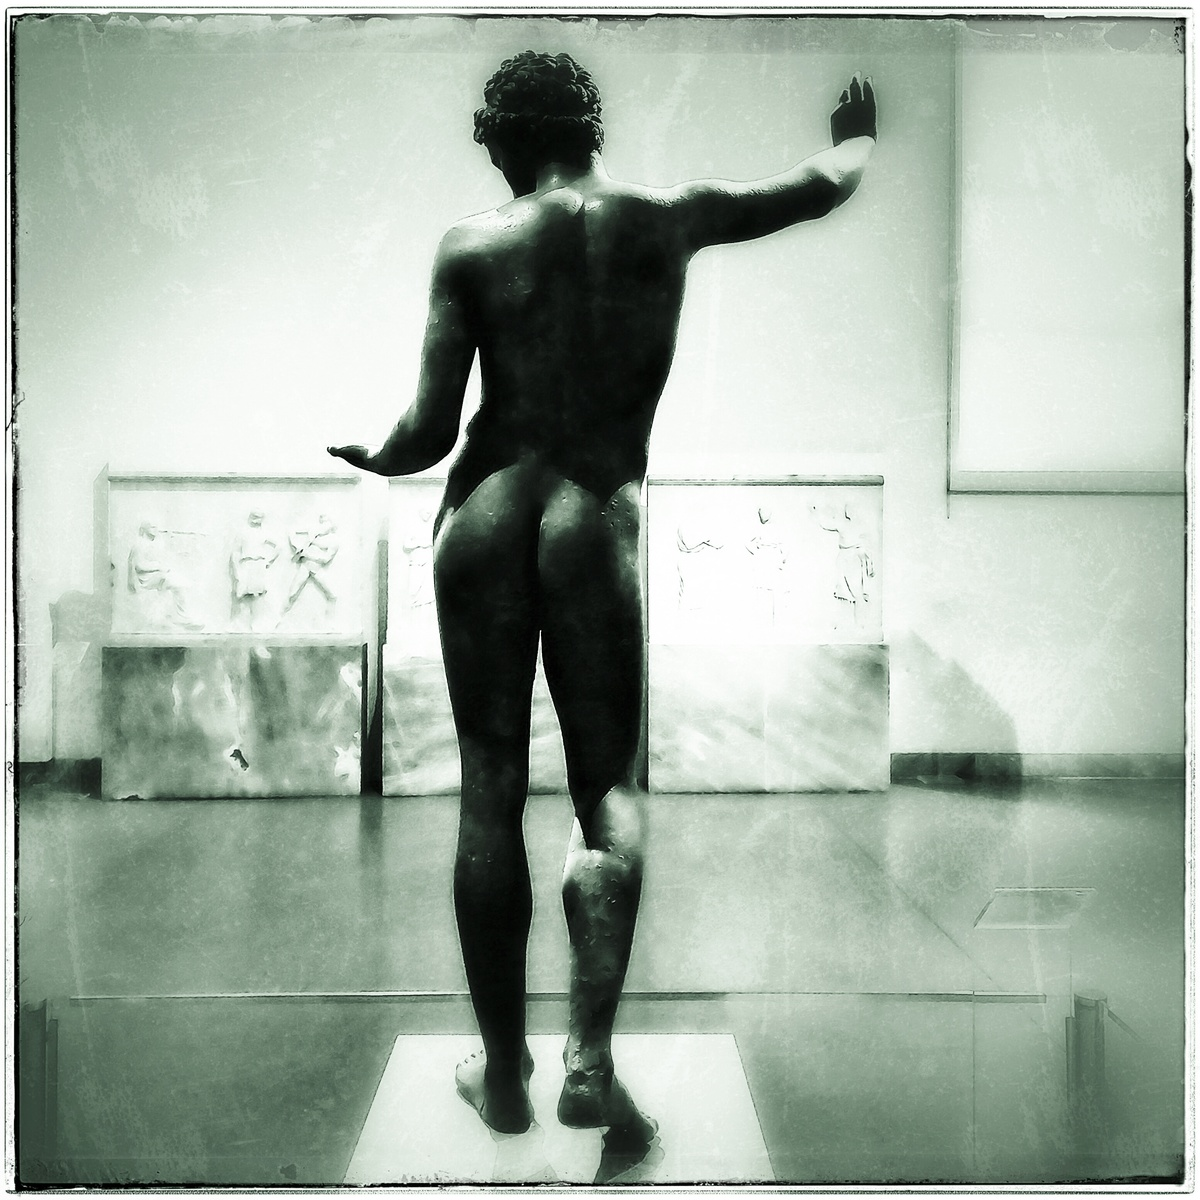
\includegraphics[width=0.8\linewidth]{thumb-lesson_VII.jpeg}
  %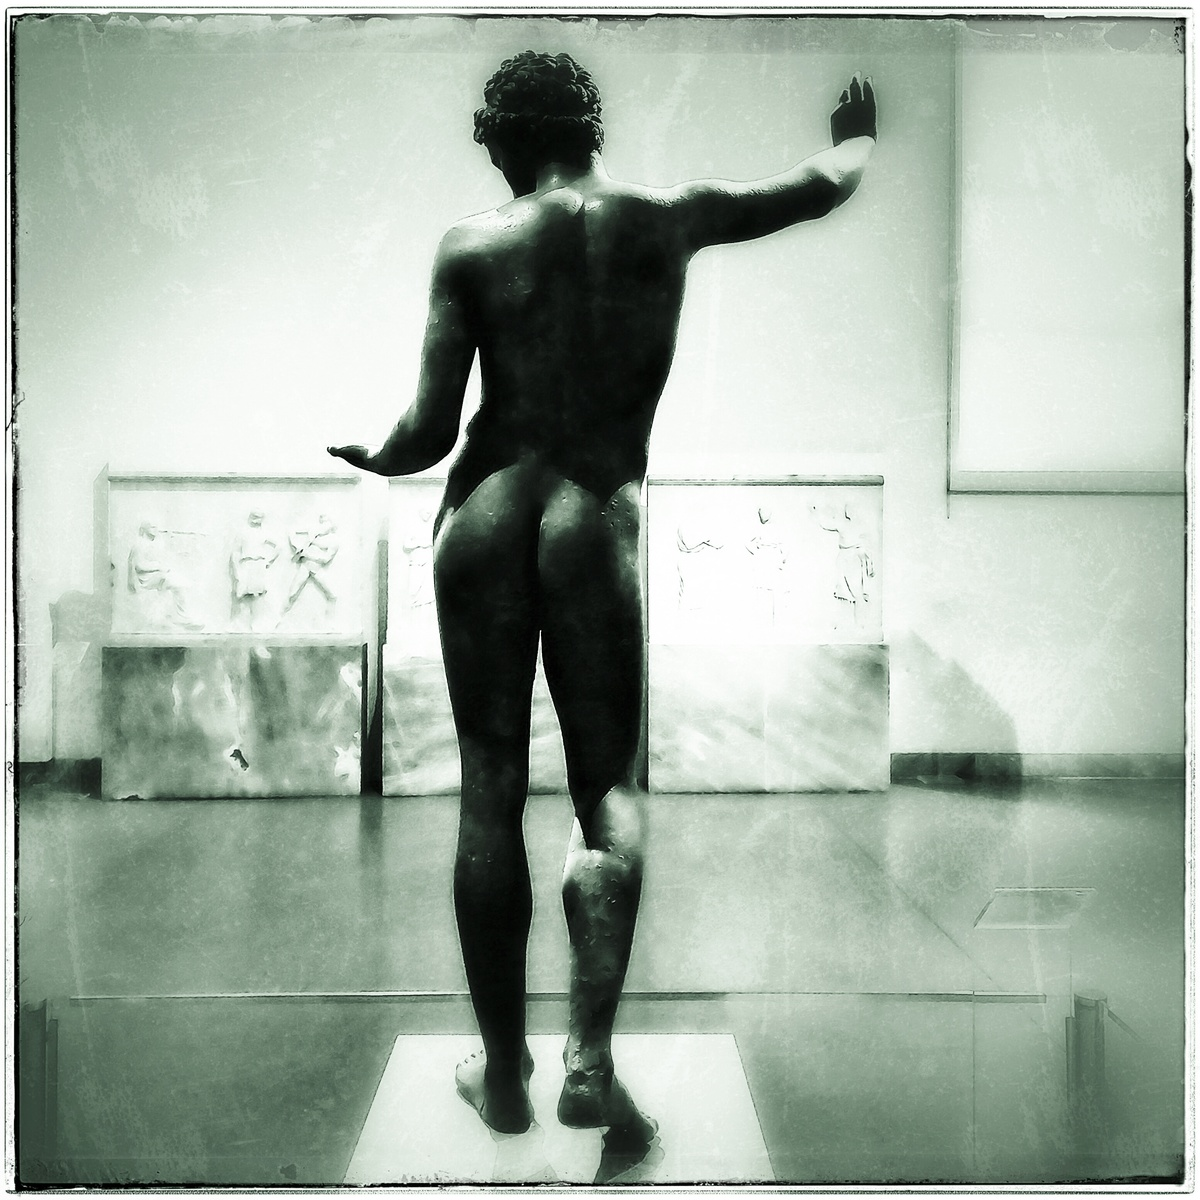
\includegraphics{thumb-lesson_VII.jpeg}
  \caption{Pavia: Almo Collegio Borromeo}
  \label{fig:textfig}
  %\zsavepos{pos:textfig}
  %\setfloatalignment{b}
\end{figure}

 

\nobibliography{latinBiblio}
\bibliographystyle{alpha}


\end{document}
